\documentclass{article}
\usepackage[utf8]{inputenc}
\usepackage{amsmath}
\usepackage{amsthm}
\usepackage{amssymb}
\usepackage{natbib}
\usepackage{graphicx}
\usepackage[utf8]{inputenc}
\usepackage[english]{babel}
\usepackage{chngcntr}

\counterwithin*{equation}{section}
\counterwithin*{equation}{subsection}
\usepackage{hyperref}
\hypersetup{
    colorlinks=true,
    linkcolor=blue,
    filecolor=magenta,      
    urlcolor=cyan,
}
\title{Solution Manual for Supplemental Psets of MIT OCW 18.02SC Fall 2010}
\author{Lu YuXun}
\date{February 2017}


\linespread{1.5}

\newtheorem{theorem}{Theorem}

\begin{document}

\maketitle

\section{Vectors and Matrices}
% Problem set 1: Vectors and Matrices
\subsection{A. Vectors}
\begin{theorem}[The Property of the Centroid of Triangles]
The centroid of a triangle is the point of intersection of its medians (the lines joining each vertex with the midpoint of the opposite side). The centroid divides each of the medians in the ratio 2:1. 
\end{theorem}
For the theorem above, refer \url{https://en.wikipedia.org/wiki/Centroid} ``Of triangle" part for details.


% Section 1A: Vectors
%
% 1A-12*
%
\textbf{1A-12*} Label the four vertices of a parallelogram in counterclockwise order as OPQR. Prove that the line segment from O to the midpoint of PQ intersects the diagonal PR in a point X that is 1/3 of the way from P to R.
\begin{figure}[htp!]
    \centering
    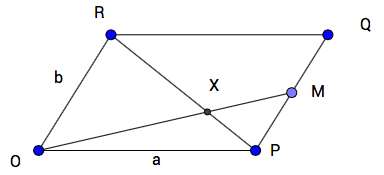
\includegraphics[width=50mm,scale=0.5]{Figure/1A-12.png}
    \caption{1A-12 Figure}
    \label{1A-12 Figure}
\end{figure}
%
% 1A-12* Solution
%
\begin{proof}
Suppose $\overrightarrow{OP} = \mathbf{a}$ and $\overrightarrow{OR} = \mathbf{b}$.
\\ We have: $\overrightarrow{RP} = \mathbf{a} - \mathbf{b}$ (1), $\overrightarrow{OM} = \mathbf{a} + \frac{1}{2} \mathbf{b}$ (2), $\overrightarrow{OX} = \mathbf{b} + \overrightarrow{RX}$ (3).
\\Let $\overrightarrow{OX} = u(\mathbf{a} + \frac{1}{2}\mathbf{b})$, $\overrightarrow{RX} = (1 - v)(\mathbf{a} - \mathbf{b})$.
\\ From (3) we can derive:
\\ $\mathbf{b} + \overrightarrow{RX} = \overrightarrow{OX} = u\mathbf{a} + \frac{u}{2}\mathbf{b} = \mathbf{b} + (1-v)\mathbf{a} - (1-v)\mathbf{b}$
that is, 
\begin{equation}
    \begin{cases}
    u = 1 - v
    \\ v = \frac{u}{2}
    \end{cases}
\end{equation}
Solve equations in (1), we have $u = \frac{2}{3}, v = \frac{1}{3}$. So $\overrightarrow{OX} = \frac{2}{3} \overrightarrow{OM}$ and $\overrightarrow{RX} = \frac{2}{3} \overrightarrow{RP}$, i.e. the intersection point X of RP and OM is 1/3 of the way from P to R.
\end{proof}
%
% 1A-13*
%
\textbf{1A-13*} a) Take a triangle $PQR$ in the plane; prove that as vectors $PQ+QR+RP = 0$.
\\ b) Continuing part a), let \textbf{A} be a vector the same length as $PQ$, but perpendicular to it, and pointing outside the triangle. Using similar vectors \textbf{B} and \textbf{C} for the other two sides, prove that \textbf{A} + \textbf{B} + \textbf{C} = \textbf{0}. (This only takes one sentence, and no computation.)
%
% 1A-13* Solution
%
\begin{proof}
a) $\because \overrightarrow{PQ} + \overrightarrow{QR} = \overrightarrow{PR}, \overrightarrow{PR} = -\overrightarrow{RP}$
\\ $\therefore \overrightarrow{PQ} + \overrightarrow{QR} + \overrightarrow{RP} = \mathbf{0}$
\\ b) Because the triangle constructed by the segment lines of \textbf{A} and \textbf{B} and \textbf{C} is the triangle $\bigtriangleup PQR$ rotated 90 degrees, since we have proved that the three vectors consisting of the three sides of $\bigtriangleup PQR$ add to \textbf{0}, \textbf{A} + \textbf{B} + \textbf{C} = \textbf{0}.
\end{proof}
%
% 1A-14*
%
\textbf{1A-14*} Generalize parts a) and b) of the previous exercise to a closed polygon in the plane which doesn't cross itself (i.e., one whose interior is a single region); label its vertices $P_1, P_2,...,P_n$ as you walk around it.
%
% 1A-14* Solution
%
\begin{proof}
We are going to use strong induction. 
\\Suppose $P(n)$: for a closed polygon with $n$ sides, $\overrightarrow{P_1P_2} + \overrightarrow{P_2P_3} + \overrightarrow{P_3P_4} + ... + \overrightarrow{P_{n-1}P_n} + \overrightarrow{P_nP_1} = \mathbf{0}$, $n \in \mathbb{N}^+ \wedge n \geq 3$.
\\ \textit{Base Case} P(3) is true, since we have proved it in \textbf{1A-13*} (a) part.
\\ \textit{Inductive Step} Suppose $P(1), P(2), ..., P(n)$ is true. For $P(n+1)$, we could add up arbitrary two adjacent vectors to eliminate one side, i.e. let $\overrightarrow{P_iP_{i+2}} = \overrightarrow{P_iP_{i+1}} + \overrightarrow{P_{i+1}P_{i+2}}$ where $ 3 \leq i \leq n+1 \wedge i \in \mathbb{N}^+$. So $P(n+1)$ decays to $P(n)$ and by our inductive assumption, $P(n)$ is true. Thus, $P(n+1)$ is true, i.e. $P(n) \implies P(n+1)$. So $P(n)$ is true for all positive nature number $n \geq 3$
\end{proof}
%
% 1A-15*
%
\textbf{1A-15*} Let $P_1, ..., P_n$ be the vertices of a regular n-gon in the plane, and $O$ its center; show without computation or coordinates that $\overrightarrow{OP_1} + \overrightarrow{OP_2} + ... + \overrightarrow{OP_n} = \mathbf{0}$.
\\ a) if $n$ is even;  b) if $n$ is odd.
%
% 1A-15* Solution
%
\begin{proof}
a) Suppose $n$ is a even number, two vectors $\overrightarrow{OP_i}$ and $\overrightarrow{OP_{i+n/2}}$ neutralized ($i \leq n/2 \wedge i \in \mathbb{N}^+$) because they have the same length/magnitude (because O is the n-gon's center) and opposite direction, thus $\overrightarrow{OP_1} + \overrightarrow{OP_2} + ... + \overrightarrow{OP_n} = \mathbf{0}$ when $n$ is a even number and $n \geq 4$.
\\ b) Suppose $n$ is an odd number, the vector $\overrightarrow{OP_i} + \overrightarrow{OP_{i+1}}$ is with the same length of the opposite vector $\overrightarrow{OP_j}$ that the point $P_j$ is opposite to the side where $\overrightarrow{OP_i}$ and $\overrightarrow{OP_{i+1}}$ towards because $\bigtriangleup P_iP_{i+1}P_j$ is a triangle and $O$ is the centroid of $\bigtriangleup P_iP_{i+1}P_j$ too. By the property of the centroid we have  $\overrightarrow{OP_j} = - (\overrightarrow{OP_i} + \overrightarrow{OP_{i+1}})$. For any n-gon that $n$ is a odd number and $n \geq 3$, for any vertex in that n-gon, there are two other different vertices of the n-gon that such three vertices form a triangle with $O$ as its centroid. Thus, $\overrightarrow{OP_1} + \overrightarrow{OP_2} + ... + \overrightarrow{OP_n} = \mathbf{0}$ where $n$ is an odd number and $n \geq 3$.
\end{proof}
%
% Section 1.2 B. Dot Product
%
\subsection{Dot Product}
%
% 1B-15*
%
\textbf{1B-15*} The \textbf{Cauchy-Schwarz inequality}
\\ a) Prove from the geometric definition of the dot product the following inequality for vectors in the plane or space; under what circumstances does equality hold?
\begin{equation}
    |\mathbf{A} \cdot \mathbf{B} | \leq |\mathbf{A}||\mathbf{B}|
\end{equation}
b) If the vectors are plane vectors, write out what this inequality says in terms of \textbf{i j}-components.
\\c) Give a different argument for the inequality (*) as follows (this argument generalizes to $n$-dimensional space):
\\i) for all values of $t$, we have (\textbf{A} + $t$\textbf{B}) $\cdot$ (\textbf{A} + $t$\textbf{B}) $\geq 0$.
\\ii) use the algebraic laws of the dot product to write the expression in (i) as a quadratic polynomial in $t$;
\\iii) by (i) this polynomial has at most one zero; this implies by the quadratic formula that its coefficients must satisfy a certain inequality - what is it?
%
% 1B-15* Solution
%
\begin{proof}
a) The component of \textbf{A} on the direction of \textbf{B} is great than or equal to the product of \textbf{A} and \textbf{B}'s lengths. The equality holds \textit{iff} \textbf{A} and \textbf{B} are in the same line, i.e. the angle between vector \textbf{A} and \textbf{B} is 180-degree or 0-degree.
\\b) Suppose $\mathbf{A} = (x_1, y_1)$ and $\mathbf{B} = (x_2, y_2)$. The equality says
\begin{equation}
    |x_1x_2 + y_1y_2| \leq \sqrt{(x_1^2 + y_1^2)(x_2^2+y_2^2)}
\end{equation}
\\c-i) Another argument for this statement is that, in any n-dimensional vector space, the length of the vectors in that vector space is great than or equal to 0.
\\c-ii) Suppose $\mathbf{A} = (x_1, x_2, x_3, ..., x_n)$ and $\mathbf{B} = (y_1, y_2, y_3, ..., y_n)$. Let $f(t) = (\mathbf{A} + t\mathbf{B})^2$, i.e. $f(t) = \sum_{i=1}^n (x_i + ty_i)^2 = \sum_{i=1}^n ( x_i^2 + t^2y_i^2 + 2tx_iy_i)$. By (i), $f(t) \geq 0$.
\\c-iii) $f(t) = t^2 \sum_{i=1}^ny_i^2 + 2t \sum_{i=1}^n x_iy_i + \sum_{i=1}^n x_i^2$. Re-write $f(t) = at^2 + bt + c$ where $c = \sum_{i=1}^n x_i^2$, $b = \sum_{i=1}^n 2x_iy_i$ and $a = \sum_{i=1}^n y_i^2$. By (i) we know $f(t) \geq 0$, then the coefficients $a,b,c$ must satisfy $b^2 - 4ac \leq 0$, i.e. $\sum_{i=1}^n (2x_iy_i)^2 - 4\sum_{i=1}^n x_i^2y_i^2 \leq 0 $. By arithmetic we know $b^2 - 4ac$ always equal to $0$, i.e. the coefficient satisfies the inequality.
\end{proof}
\end{document}